\section{Exercise 3}

\subsection{Instruction}

\begin{figure}[H]
	\centering
	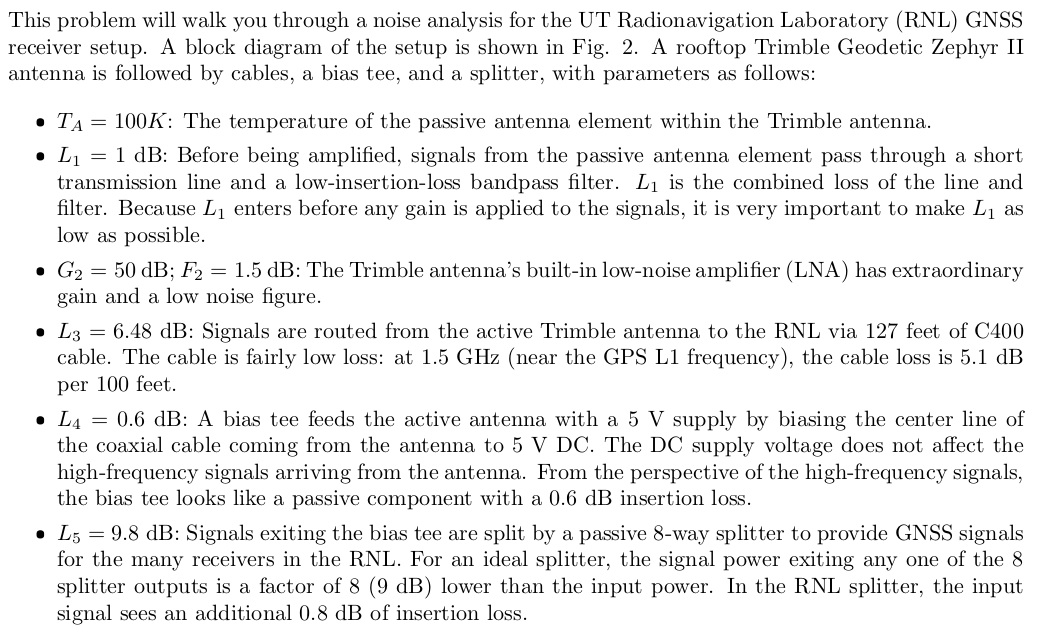
\includegraphics[width=0.9\textwidth]{figs/ex3_instructions.png}
\end{figure}

\begin{figure}[H]
	\centering
	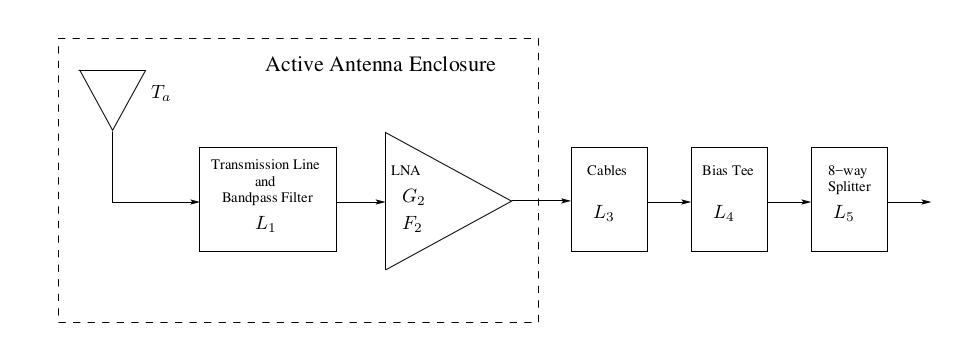
\includegraphics[width=0.9\textwidth]{figs/ex3_diagram.png}
	\caption{Radionavigation Laboratory GNSS receiver setup.}
	\label{fig:ex3_diagram}
\end{figure}

\subsection{Results}

\subsubsection{Item a}

Calculate the noise figure $F_1$ and effective input temperature $T_1$
corresponding to $L_1$. Assume an input temperature $T_{in} = T_0 = 290K$.

Since $L_1$ is a passive element

\begin{equation}
	F = \frac{1}{G} > 1
\end{equation}

\begin{equation}
	T_E = \frac{1 - G}{G} T_0
\end{equation}

Therefore, $F_1 = 1.259$ and $T_1 = 75.11 K$.

\subsubsection{Item b}

Calculate the effective input temperature $T_2$ corresponding to $F_2$. Assume
$F_2$ is taken from a device data sheet that assumes $T_{in} = T_0 = 290K$.

\begin{equation}
	T_2 = (F_2 - 1) T_0
\end{equation}

Therefore, since $F_2 = 1.5dB = 1.413$ the effective input temperature
$T_1 = 119.64 K$.

\subsubsection{Item c}

Lump losses $L_3$, $L_4$, and $L_5$ into a single loss $L_{345}$. Calculate an
effective input temperature $T_{345}$ corresponding to $L_{345}$. Assume an
input temperature $T_{in} = T_0 = 290K$.

Since, $L_3 = 6.48 dB$, $L_4 = 0.6 dB$, and $L_5 = 9.8 dB$ the lump losses are
$L_{345} = 16.88 dB$. The equivalent system is passive.
Thus, $F = L = 48.75$.

\begin{equation}
	T_{345} = (F_{345} - 1) T_0
\end{equation}

Consequently, $T_{345} = 13,848.3 K$

\subsubsection{Item d}

Use the Friis formula to calculate the system temperature $T_S = T_A + T_R$,
expressed in degrees K. How many degrees K do the combined losses $L_{345}$
contribute to the system temperature?

\begin{equation}
	T_R = T_1 + \frac{T_2}{G_1} + \frac{T_{345}}{G_1 G_2}
\end{equation}

\begin{equation}
	T_R = 75.11 + \frac{119.64}{0.794} + \frac{13,848.3}{0.794*100000}
	= 75.11 + 150.68 + 0.17
	= 293.28 K
\end{equation}

Therefore, $T_S = T_A + T_R = 393.28 K$. Notice that the combined losses
$L_{345}$ contribute $0.17 K$ to the overall system temperature.

\subsubsection{Item e}

The effective noise floor of the whole cascade, $N_0$, is related to the system
temperature $T_S$ by $N_0 = k * T_S$, where $k$ is Boltzmann’s constant, equal
to $-228.6 dBW/K-Hz$. The quantity $N_0$ is the one used in calculating $C/N_0$,
that all-important parameter in GNSS receiver design. For purposes of
calculating $C/N_0$, you can think of the receiver cascade as a chain of ideal
gain blocks (no internal noise) with an effective noise density $N_0$ at the
beginning of the cascade (i.e., at the output of the passive antenna element
just before the $L_1$ block). This is precisly the point where the signal power
$C$ is defined, so it makes sense to calculate the ratio $C/N_0$ here. Calculate
the value of $N_0$ in $dBW/Hz$. For an expected GPS $L_1$ C/A received signal
power $C$ ranging from $-162.5$ to $-154.5 dBW$, calculate the expected range of
carrier-to-noise ratio $C/N_0$ values. Express your result in $dB-Hz$.

If one thinks the receiver cascade as a chain of ideal gain blocks (no internal
noise). Then $T_S = T_A = 20 dBK$

\begin{equation}
	N_0 = k*T_S = -228.6 \frac{dBW}{K-Hz} + 20 dBK = -208.6 \frac{dBW}{Hz}
\end{equation}


\begin{equation}
	46.1 dB-Hz = -162.5 - (-208.6) < \frac{C}{N_0} < -154.5 - (-208.6) = 54.1 dB-Hz
\end{equation}

\subsubsection{Item f}

What is the noise floor $N_{0,sp}$ at the output of the 8-way splitter?
Express your answer in dBW/Hz.

Since $T_S = 393.28 K = 25.947 dBK$

\begin{equation}
	N_0 = k*T_S = -228.6 \frac{dBW}{K-Hz} + 25.947 dBK = -202.65 \frac{dBW}{Hz}
\end{equation}
